\section{Introducción}
{
% Debe mencionar las motivaciones de realizar este proyecto, definir sus objetivos, qué busca
% resolver o demostrar y una explicación general del trabajo realizado.

% Contexto de las noticias actualmente
En la actualidad, los usuarios del internet se encuentran constantemente bombardeados de información y noticias, proveniente de fuentes que parecen diversificarse día a día. 

% Importancia para resolver esto
Es por ello, que no siempre se puede identificar con certeza cuando una noticia es verdadera o falsa. Lo cual cobra importancia, ya que las noticias son la forma principal en que las personas pueden entender el contexto en que están viviendo y formar sus opiniones. Además de que las noticias falsas son una forma maliciosa de propagar desinformación para manejar la opinión pública en beneficio de sus creadores. 

% Objetivo
Es por esto que el objetivo de este trabajo será desarrollar una herramienta que permita \textbf{clasificar} una noticia como verdadera o falsa, en base al título y cuerpo de la noticia.

Para esto, se utilizarán diversas herramientas clásicas de Aprendizaje de Máquinas, como lo es Procesamiento de Lenguaje Natural y Clasificación Binaria. Es específico se usará vectorización, análisis léxico y lematización sintáctica para procesar el texto, y luego modelos como Naïve Bayes, Regresión Logística y Perceptrón para la clasificación. 

% Origen de los datos
% Para esto, se obtendrán diversas noticias de US a través de 
% \href{https://www.kaggle.com/clmentbisaillon/fake-and-real-news-dataset}{kaggle}, etiquetadas por verdaderas o falsas. 

}

\section{Marco Teórico}
{
\subsection{Herramientas de NLP}
El procesamiento del lenguaje natural investiga el uso de computadores para procesar o entender el lenguaje humano (natural) con el objetivo de realizar tareas útiles. Dentro de las aplicaciones más comunes están: reconocimiento de voz, interpretación del lenguaje hablado (SLU por sus siglas en inglés), sistemas de diálogos, análisis léxico, análisis gramatical, análisis sintáctico, análisis morfológico, traducciones, recuperación de texto, análisis de sentimientos, etc. 

Uno de las herramientas más importantes en el procesamiento de textos, es la vectorización. Ya que permite a la máquina entender el contenido simbólico a través de representaciones numéricas significativas. En el caso de la técnica usada, construye una matriz para registrar la frecuencia de cada componente léxico observado. 

Sin embargo, el trabajo requerido para convertir el texto natural en componentes léxicos que puedan aportar significado  la matriz no es trivial. Se ocupan técnicas de análisis léxico, análisis sintáctico y lematización. 

\begin{itemize}
    \item El \textbf{análisis léxico} del texto, corresponde a dividir oraciones o párrafos en componentes léxicos o símbolos, para así poder visualizar individualmente las palabras o símbolos que componen una secuencia de texto. 
    \item Luego, la \textbf{lematización} es el proceso mediante el cual las palabras de un texto que pertenecen a un mismo paradigma flexivo o derivativo son llevadas a una forma normal que representa a toda la clase. Esta forma normal, llamada lema, es típicamente la palabra utilizada como entrada en los diccionarios de lengua. 
    \item En la lematización usada, se necesita distinguir si la palabra es un verbo, sustantivo, adjetivo o adverbio, para llevar a su raíz más exacta. Dicho proceso es el \textbf{análisis sintáctico}. 
\end{itemize}

Así, cada componente léxico corresponde a un lema. Lo cual permite agrupar de mejor manera las palabras por significado y otorga mayor importancia a cada representación en la vectorización. 

}

\section{Descripción de los Datos}
{
\subsection{Descripción del dataset}
La base de datos se obtuvieron a partir de Kaggle, del \textit{dataset} llamado ``\href{https://www.kaggle.com/clmentbisaillon/fake-and-real-news-dataset}{Fake and 
real news dataset}''.

Esta base de datos consiste en dos \textit{datasets}: el de noticias falsas (17.903 datos) y el de noticias verdaderas (20.826 datos). Ambos datasets 
comparten las mismas columnas: \textit{title}, \textit{text}, \textit{subject} y \textit{date}. Estas corresponden al titular de
la noticia, al contenido de la noticia, al tipo de noticia que es y la fecha de la noticia, respectivamente.

Las columnas \textit{title} y \textit{text} son de tipo cadena; \textit{subject} es un tipo de dato categórico y \textit{date}
es un tipo de dato temporal. 

% \subsubsection{Descripción de las categorías de la columna \textit{subject}}
En el \textit{dataset} de las noticias verdaderas, existen dos etiquetas para la columna \textit{subject}, las cuales son \textbf{politicsNews} y \textbf{worldnews}. La etiqueta \textbf{politicsNews} posee 11.272 datos y es para referirse a las noticias que tengan una connotación política, mientras que la etiqueta \textbf{worldnews} posee 10.145 datos y es para referirse a las noticias que ocurren fuera de EE.UU.

Mientras que el \textit{dataset} de las noticias falsas, posee seis etiquetas:
\textbf{News}, \textbf{politics}, \textbf{Government News}, \textbf{left-news}, \textbf{US news} y \textbf{Middle-east}. A continuación se dará una breve descripción de cada categoría:
\begin{itemize}
    \item La etiqueta de \textbf{News} posee 9.050 datos y corresponde a las noticias estándar,
    \item La de \textbf{politics} posee 6.836 datos y corresponde a noticias de connotación política,
    \item La de \textbf{Government News} posee 1.568 datos y corresponde a noticias sobre el gobierno,
    \item La de \textbf{left-news} posee 4.456 datos y corresponde a noticias del espectro de la izquierda política,
    \item La de \textbf{US News} posee 784 datos y corresponde a noticias sobre EE.UU., y finalmente
    \item La de \textbf{Middle-east} posee 778 datos y corresponde a noticias del Oriente Medio.
\end{itemize}

El \textit{dataset} originalmente no posee valores nulos. Sin embargo, el \textit{dataset} de las noticias falsas posee 10 datos etiquetados como fecha, a pesar de que no lo sean.


\subsection{Tratamiento de los Datos}

\subsubsection{Limpieza del dataset}
Se crea una nueva columna en ambos \textit{datasets}, llamada \textit{true}, el cual determina si la noticia es verdadera o falsa. Se le asigna a todas las noticias verdaderos, el valor de true igual a $1$, y $0$ a las noticias falsas. Paso siguiente, se concatenan ambos \textit{datasets}. Además, se marcan los datos que no sean fechas de la columna \textit{date} por el tipo de dato llamado \textit{Not a Time}, y se eliminan los datos nulos que posea el \textit{dataset}.

\subsubsection{Procesamiento de los datos}
Luego, se procede a procesar la información de tipo texto (esto es, para las columnas \textit{title} y \textit{text}) a través de NLP. Se escoge una muestra aleatoria de 2500 filas\footnote{Si se escogen más filas, la memoria para guardar la información del computador queda sobrecargada} de los datasets originales (para las noticias verdaderas y falsas) y se empieza transformando el texto de las cadenas en minúsculas. 

Luego se realiza un análisis léxico (a.k.a. \textit{tokenization}), y por cada componente léxica (a.k.a. \textit{token}), si es que no corresponde a una \textit{stopword}, se lematiza la componente léxica. Realizada la lematización de cada componente léxica, se procede a unir nuevamente todas las componentes en un único texto de tipo cadena.

Paso seguido, este nuevo texto generado se reemplaza en una copia del \textit{dataset}, en el lugar dónde estaba la información no procesada originalmente.

Finalmente, se empieza a codificar la información a través de un vector de características. 

\subsection{Análisis Exploratorio de los Datos}

\begin{figure}
\centering
\begin{subfigure}{\escala\textwidth}
    \centering
    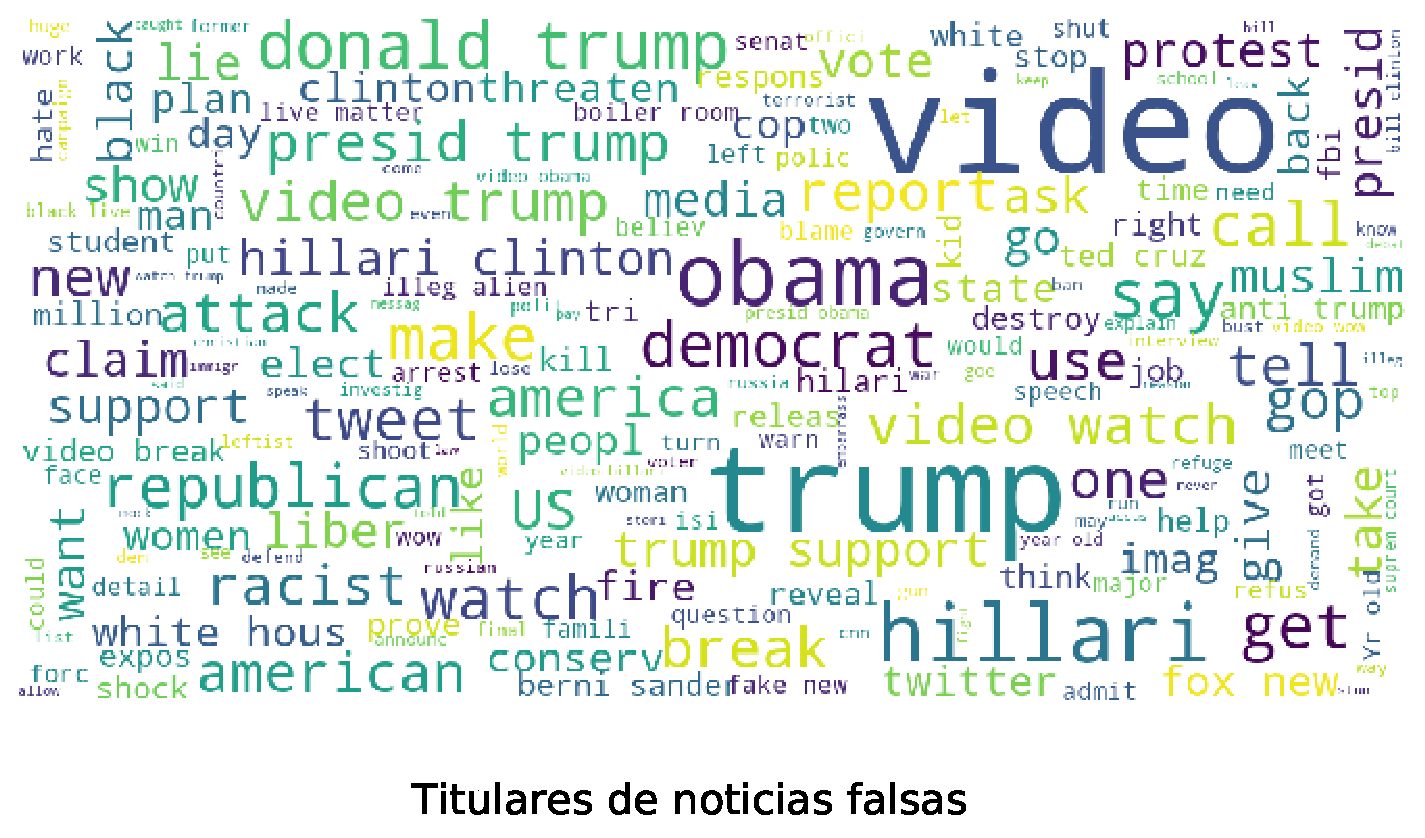
\includegraphics[width=\textwidth]{imagenes/wordcloud_titulares_falsas.pdf}
    \caption{Titulares de noticias falsas}
    \label{fig:tit-fake}
\end{subfigure}%
\newline
\begin{subfigure}{\escala\textwidth}
    \centering
    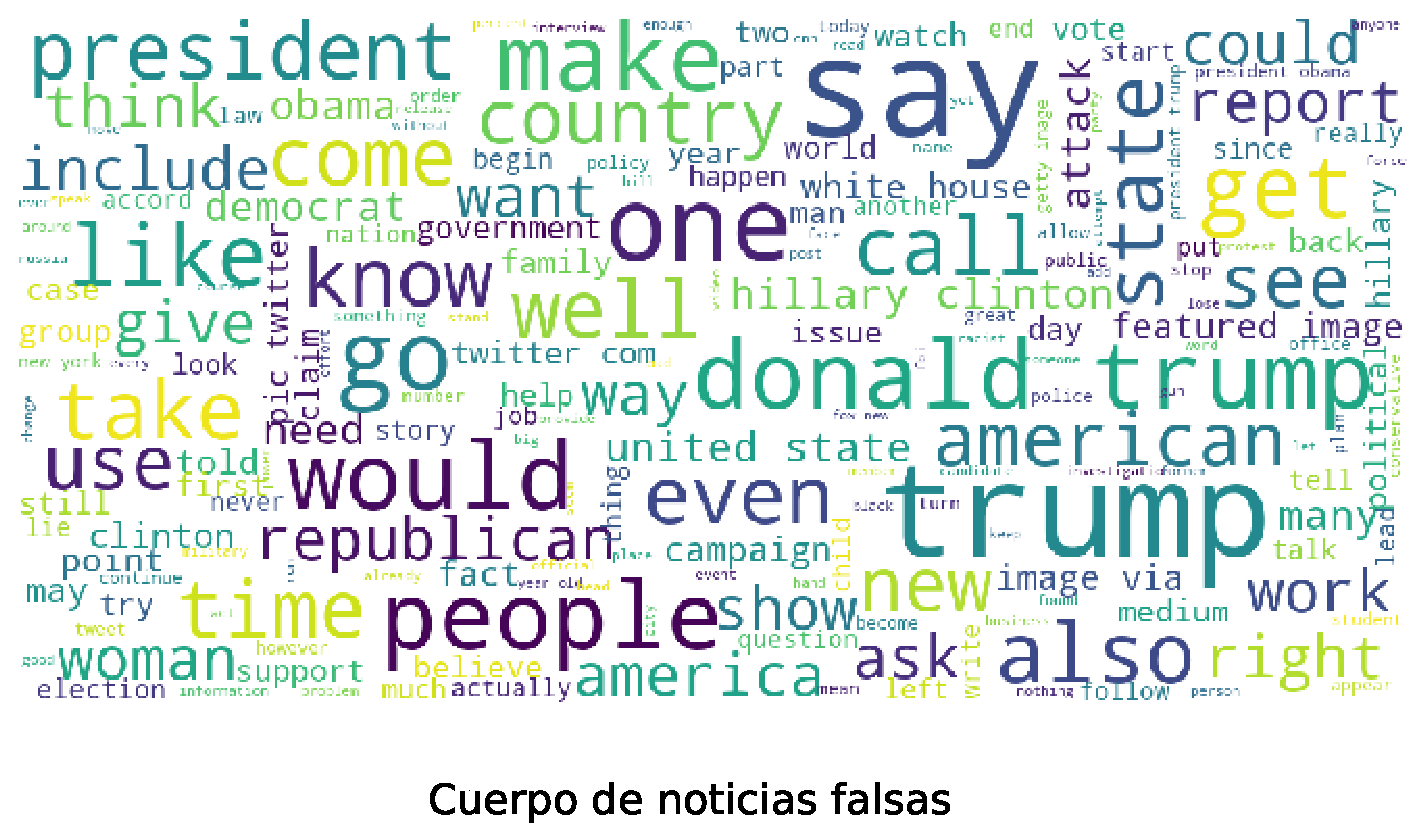
\includegraphics[width=\textwidth]{imagenes/wordclouds_cuerpo_falsas.pdf}
    \caption{Cuerpo de noticias falsas}
    \label{fig:text-fake}
\end{subfigure}
\caption{Nube de palabras para las noticias falsas.}
\label{fig:fake}
\end{figure}
En las figuras \ref{fig:tit-fake} y \ref{fig:text-fake} de observan nubes de palabras realizadas a partir de los titulares y el cuerpo de las noticias falsas. A partir de ellas, se concluye que las temáticas principales de las noticias falsas son: videos, Trump, Obama, Hillary, ataque, racista, presidente, mujer, republicanos, demócratas, musulmán, blanco, negro, terrorista, mentira, etc. Que corresponden a figuras políticas y temas sensibles de discriminación. 

\begin{figure}
\centering
\begin{subfigure}{\escala\textwidth}
    \centering
    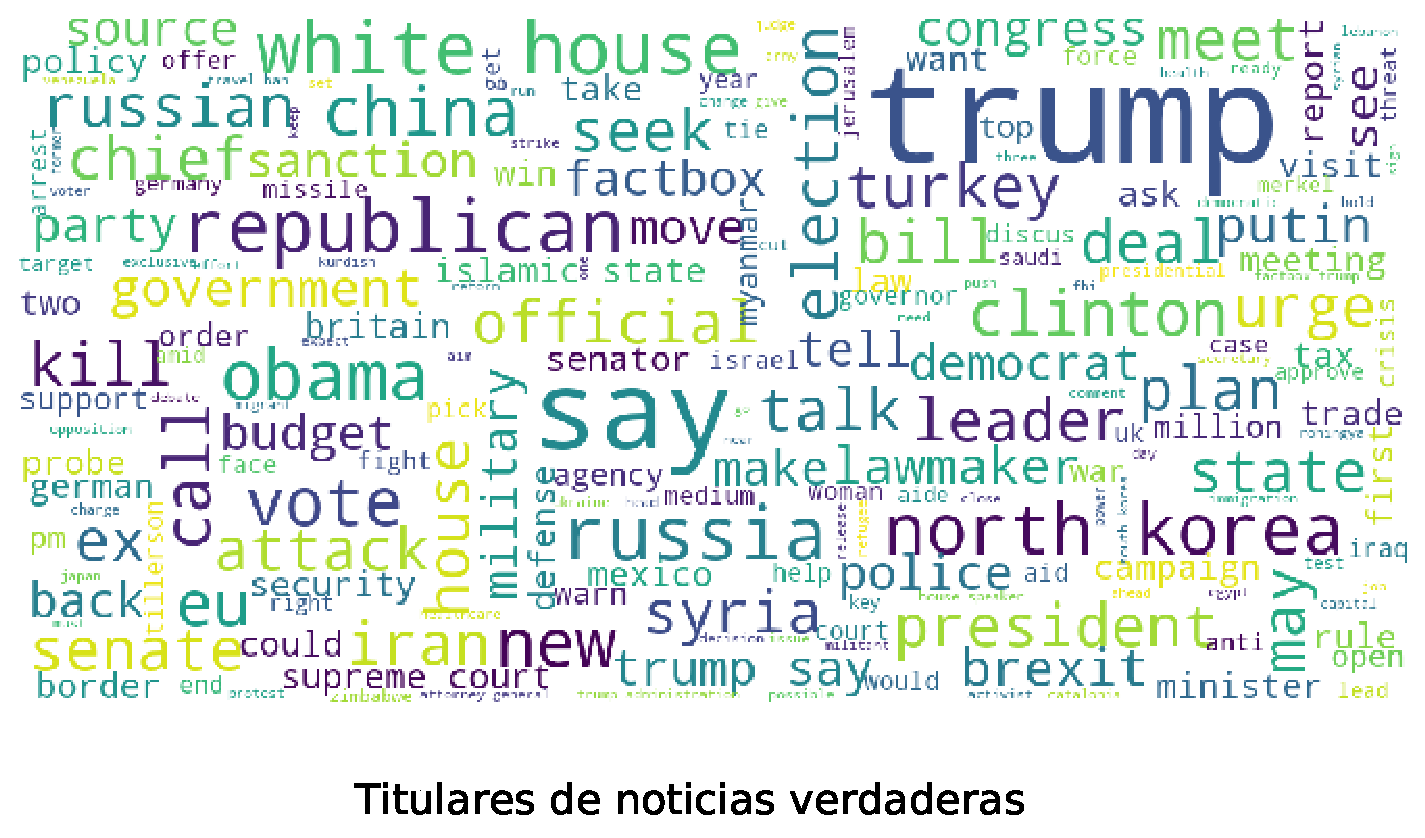
\includegraphics[width=\textwidth]{imagenes/wordcloud_titulares_verdaderas.pdf}
    \caption{Titulares de noticias verdaderas}
    \label{fig:tit-true}
\end{subfigure}%
\newline
\begin{subfigure}{\escala\textwidth}
    \centering
    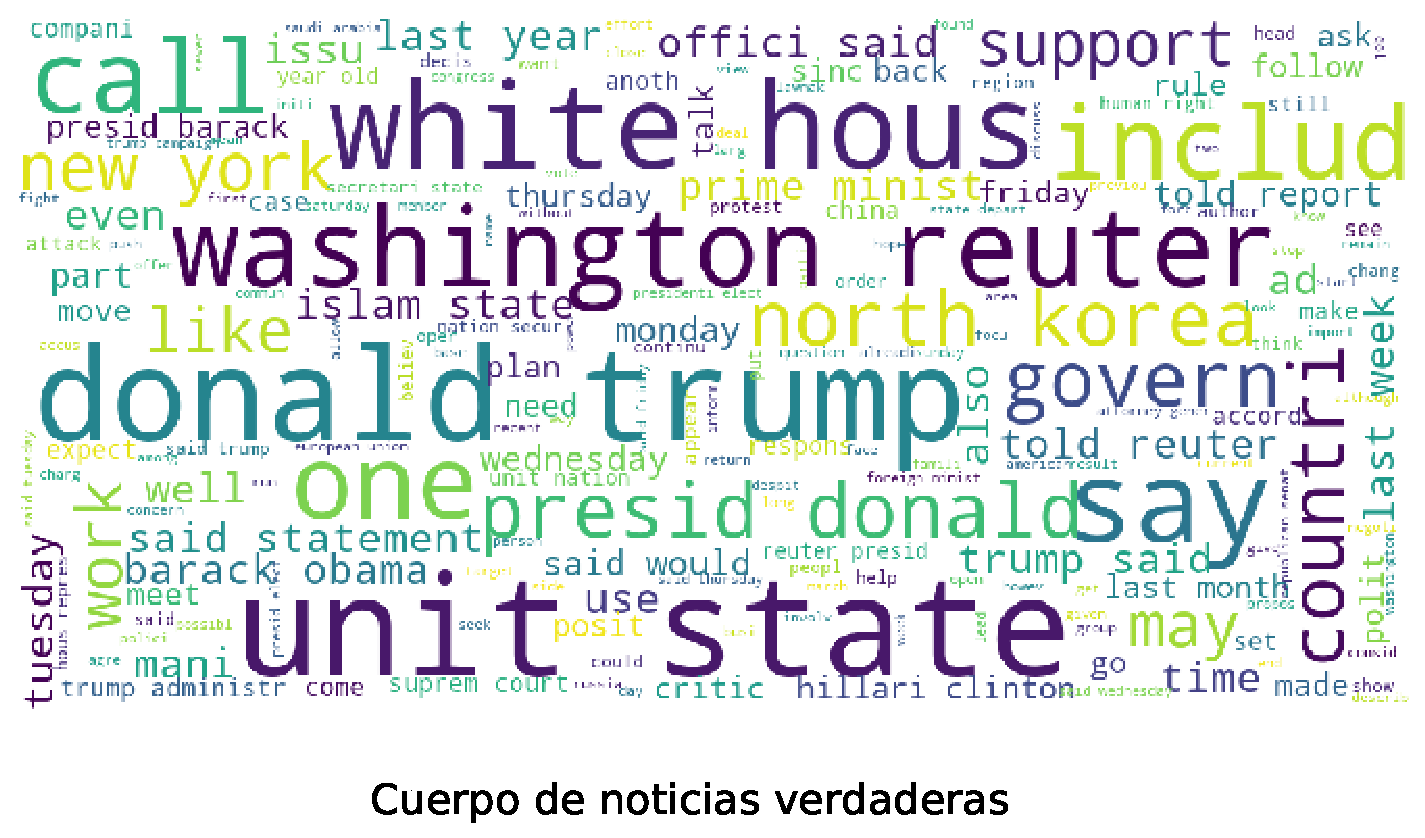
\includegraphics[width=\textwidth]{imagenes/wordclouds_cuerpo_verdaderas.pdf}
    \caption{Cuerpo de noticias verdaderas}
    \label{fig:text-true}
\end{subfigure}
\caption{Nube de palabras para las noticias verdaderas.}
\label{fig:true}
\end{figure}
Mientras que en \ref{fig:tit-true} y \ref{fig:text-true} las palabras mayoritarias son: Trump, Casa blanca, Rusia, China, Obama, gobierno, EEUU., Corea del Norte, Turquía, elección, muerte, voto, Clinton, lider, etc. Es decir, son noticias orientadas a las relaciones internacionales, y no abordan temas tan polémicos como las noticias falsas. 


\begin{figure}
    \centering
    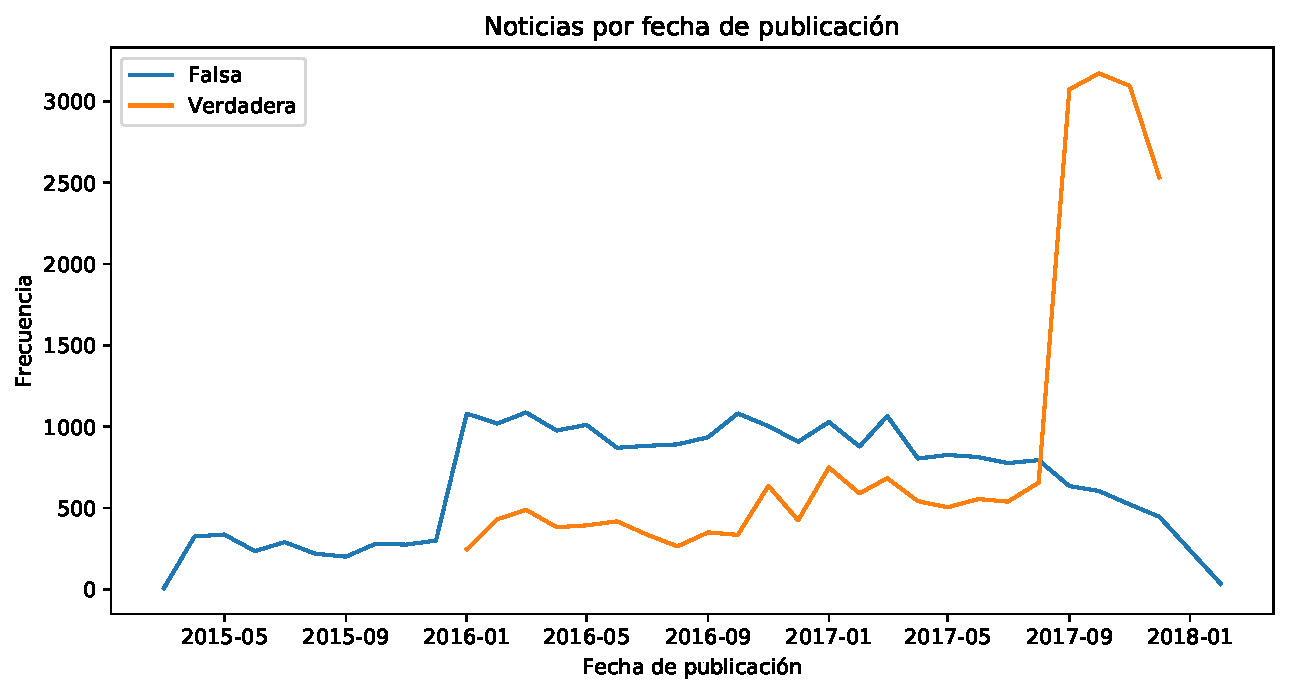
\includegraphics[width=0.47\textwidth]{imagenes/noticias_fecha_publicacion.pdf}
    \caption{Frecuencia de noticias por fecha de publicación}
    \label{fig:not-fecha-pub}
\end{figure}

}

\section{Metodología}
{
\subsection{Modelos}
Se escogerán cuatro modelos modelos:  \textit{Naïve Bayes} (NB), por su simpleza, \textit{Regresión Logística} (RL), el \textit{Perceptrón}, ambos modelos por su capacidad de predecir sin utilizar técnicas geométricas, y \textit{Support Vector Classifier} (SVC)

\subsubsection{Preparación del modelo de NB} 
Se escogerá un prior uniforme para Naïve Bayes.

\subsubsection{Preparación del modelo de RL}
No se ajustarán hiperparámetros para este modelo.

\subsubsection{Preparación del modelo de Perceptrón}
No se ajustarán hiperparámetros para este modelo.

\subsection{Preparación del Conjunto de Entrenamiento y Test}
Luego de procesada toda la información del texto, se escoge una columna para realizar la predicción. En nuestro caso, se escogen las columnas \textit{title}, \textit{text} (ambas por separado) y una concatenación de \textit{title} $+$ \textit{text}. 

Fijada una columna, se procede a dividir de forma aleatoria un $70\%$ de los datos para el entrenamiento, y un $30\%$ de los datos para el test.

}

\section{Resultados}
{
En la Tabla \ref{tab:resumen} se puede observar el porcentaje de precisión que resultó después de utilizar los tres modelos en cada una de las columnas.
\begin{table}
\centering
\caption{Tabla de Resumen}
\label{tab:resumen}
\begin{tabular}{rccc}
\toprule
 title &   text &  title and text \\
\midrule
 89.87 &  99.19 &           98.92 \\
 89.13 &  98.92 &           98.92 \\
 89.80 &  98.78 &           98.58 \\
\bottomrule
\end{tabular}
\end{table}


}

\section{Discusión y Conclusiones}
{

Observamos a partir de la Tabla \ref{tab:resumen} que, ocupando el modelo de \textit{Regresión Logística} sobre la columna de \textit{text} (procesada) es la que resulta con la mayor precisión entre todas combinaciones. 

Sin embargo, es destacable que ocupando únicamente el titular de la noticia, todos los modelos tengan aproximadamente un $90\%$ de precisión a la hora de predecir la veracidad de la misma. Lo cuál significa que, basta con recibir el titular de una noticia para determinar con bastante precisión si ésta es verdadera o falsa.

Además, es destacable que utilizando el titular de la noticia, junto con el texto de la misma, termina empeorando la calidad de la predicción en los tres modelos. Esto resulta contra intuitivo, pues se espera que añadiendo ``más información'' que puede resultar útil, realmente termine perjudicando la calidad de predicción.

\subsection{Futuras Mejoras}

Observamos que la división entre el conjunto de entrenamiento y de test no es la mejor forma de particionar los datos. Más que nada por el siguiente hecho: los datos son dependientes del tiempo. 

Esta dependencia temporal es lo que obliga a considerar el escenario de, ``estoy ocupando los datos del pasado para predecir el futuro'', con lo que una forma óptima de particionar los datos es la siguiente: ordenar los datos por fecha, y luego, dividir los primeros $x\%$ de los datos para el conjunto de entrenamiento, y los restantes $(100-x)\%$ como conjunto de test.
}

% \section{Desarrollo}
% {
% % El procedimiento y los experimentos realizados, descripción de los datos, la metodología usada, las
% % configuraciones (parámetros) de los algoritmos usados, etc. Explicar las decisiones que tomaron y el porqué. Si
% % usaron un algoritmo para resolver el problema, explicar su elección y por qué no otro. No es necesario que sea
% % una explicación rigurosa, puede ser por la naturaleza del problema, de forma intuitiva o por aspectos prácticos
% \subsection{Descripción de los datos}
% {
% Los datos se obtuvieron de la Base de Datos \href{https://www.kaggle.com/clmentbisaillon/fake-and-real-news-dataset}{Fake and 
% real news dataset}, de kaggle. 

% Este consiste en dos datasets: el de noticias falsas (17903 datos) y el de noticias verdaderas (20826 datos). Ambos datasets 
% comparten las mismas columnas: \textit{title}, \textit{text}, \textit{subject} y \textit{date}. Estas corresponden al titular de
% la noticia, al contenido de la noticia, al tipo de noticia que es y la fecha de la noticia, respectivamente.

% Las columnas \textit{title} y \textit{text} son de tipo cadena; \textit{subject} es un tipo de dato categórico y \textit{date}
% es un tipo de dato temporal. 
% }
% }

% \section{Resultados y Análisis}
% {
% % Mostrar, explicar y discutir los resultados obtenidos. El análisis incluye una interpretación superficial (funcionó/no funcionó), y también un análisis de si era o no lo esperado, por qué, y qué
% % se podría mejorar
% \lipsum[3]
% }

% \section{Conclusión}
% {
% % Las conclusiones que se obtienen del proyecto (No ponga conclusiones del estilo ”aprendí mucho”).
% % Incluya las dificultades que se encontraron y propuestas de trabajo a futuro.
% \lipsum[4]
% }